\documentclass[10pt,twocolumn,letterpaper]{article}
\usepackage{cvpr}
\usepackage{times}
\usepackage{epsfig}
\usepackage{url}
\usepackage{graphicx}
\usepackage{amsmath}
\usepackage{amssymb}
\usepackage[breaklinks=true,bookmarks=false,backref=page]{hyperref}
\cvprfinalcopy
\def\cvprPaperID{****}
\def\httilde{\mbox{\tt\raisebox{-.5ex}{\symbol{126}}}}
\begin{document}
\title{\textbf{Unsupervised Representation Learning with Deep Convolutional
		Generative Adversarial Networks}}
\author{Liangjie Cao\\\\ July 18, 2018}
\maketitle
\abstract{In recent years, supervised learning with convolutional networks (CNNs) has seen huge adoption in computer vision applications. Comparatively, unsupervised learning with CNNs has received less attention. In this work we hope to help bridge the gap between the success of CNNs for supervised learning and unsupervised learning. We introduce a class of CNNs called deep convolutional generative adversarial networks (DCGANs), that have certain architectural constraints, and demonstrate that they are a strong candidate for unsupervised learning. Training on various image datasets, we show convincing evidence that our deep convolutional adversarial pair learns a hierarchy of representations from object parts to scenes in both the generator and discriminator. Additionally, we use the learned features for novel tasks demonstrating their applicability as general image representations.}
\section{Introduction}
Learning reusable feature representations from large unlabeled datasets has been an area of active research. In the context of computer vision, one can leverage the practically unlimited amount of unlabeled images and videos to learn good intermediate representations, which can then be used on
a variety of supervised learning tasks such as image classification. The authors propose that one way to buildgood image representations is by training Generative Adversarial Networks (GANs)~\cite{name1}, and later reusing parts of the generator and discriminator networks as feature extractors for supervised tasks. GANs provide an attractive alternative to maximum likelihood techniques. One can additionally argue that their learning process and the lack of a heuristic cost function (such
as pixel-wise independent mean-square error) are attractive to representation learning. GANs have been known to be unstable to train, often resulting in generators that produce nonsensical outputs.
There has been very limited published research in trying to understand and visualize what GANs learn, and the intermediate representations of multi-layer GANs.
\section{Reated Work}
\subsection{Representation Learning from Unlabeled Data}
Unsupervised representation learning is a fairly well studied problem in general computer vision research, as well as in the context of images. A classic approach to unsupervised representation learning is to do clustering on the data (for example using K-means), and leverage the clusters for improved classification scores. In the context of images, one can do hierarchical clustering of image patches~\cite{name2} to learn powerful image representations. Another popular method is to train auto-encoders (convolutionally, stacked~\cite{name3}, separating the what and where components of the code~\cite{name4}, ladder structures~\cite{name5}) that encode an image into a compact code, and decode the code to reconstruct the image as accurately
as possible. These methods have also been shown to learn good feature representations from image pixels. Deep belief networks have also been shown to work well in learning hierarchical representations.
\subsection{Generating Natural Images}
Generative image models are well studied and fall into two categories: parametric and non-parametric.
\par The non-parametric models often do matching from a database of existing images, often matching patches of images, and have been used in texture synthesis, super-resolution and in-painting.
\par Parametric models for generating images has been explored extensively (for example on MNIST digits or for texture synthesis~\cite{name6}). However, generating natural images of the real world have had not much success until recently. Generative Adversarial Networks generated
images suffering from being noisy and incomprehensible. A recurrent network
approach  and a deconvolution network approach have also recently had some success with generating natural images. However, they have not leveraged the generators for supervised tasks.
\subsection{Visualizing the Internals of CNNs}
One constant criticism of using neural networks has been that they are black-box methods, with little understanding of what the networks do in the form of a simple human-consumable algorithm. In the
context of CNNs, Zeiler \emph{et. al.}~\cite{name7} showed that by using deconvolutions and filtering the maximal activations, one can find the approximate purpose of each convolution filter in the network. Similarly, using a gradient descent on the inputs lets us inspect the ideal image that
activates certain subsets of filters.
\section{Approach and Architecture}
Historical attempts to scale up GANs using CNNs to model images have been unsuccessful. This motivated the authors of LAPGAN to develop an alternative approach to iteratively upscale low resolution generated images which can be modeled more reliably. They also encountered difficulties attempting to scale GANs using CNN architectures commonly used in the
supervised literature. However, after extensive model exploration we identified a family of architectures that resulted in stable training across a range of datasets and allowed for training higher resolution and deeper generative models.
\begin{figure}[!htb]
   	\centering
   	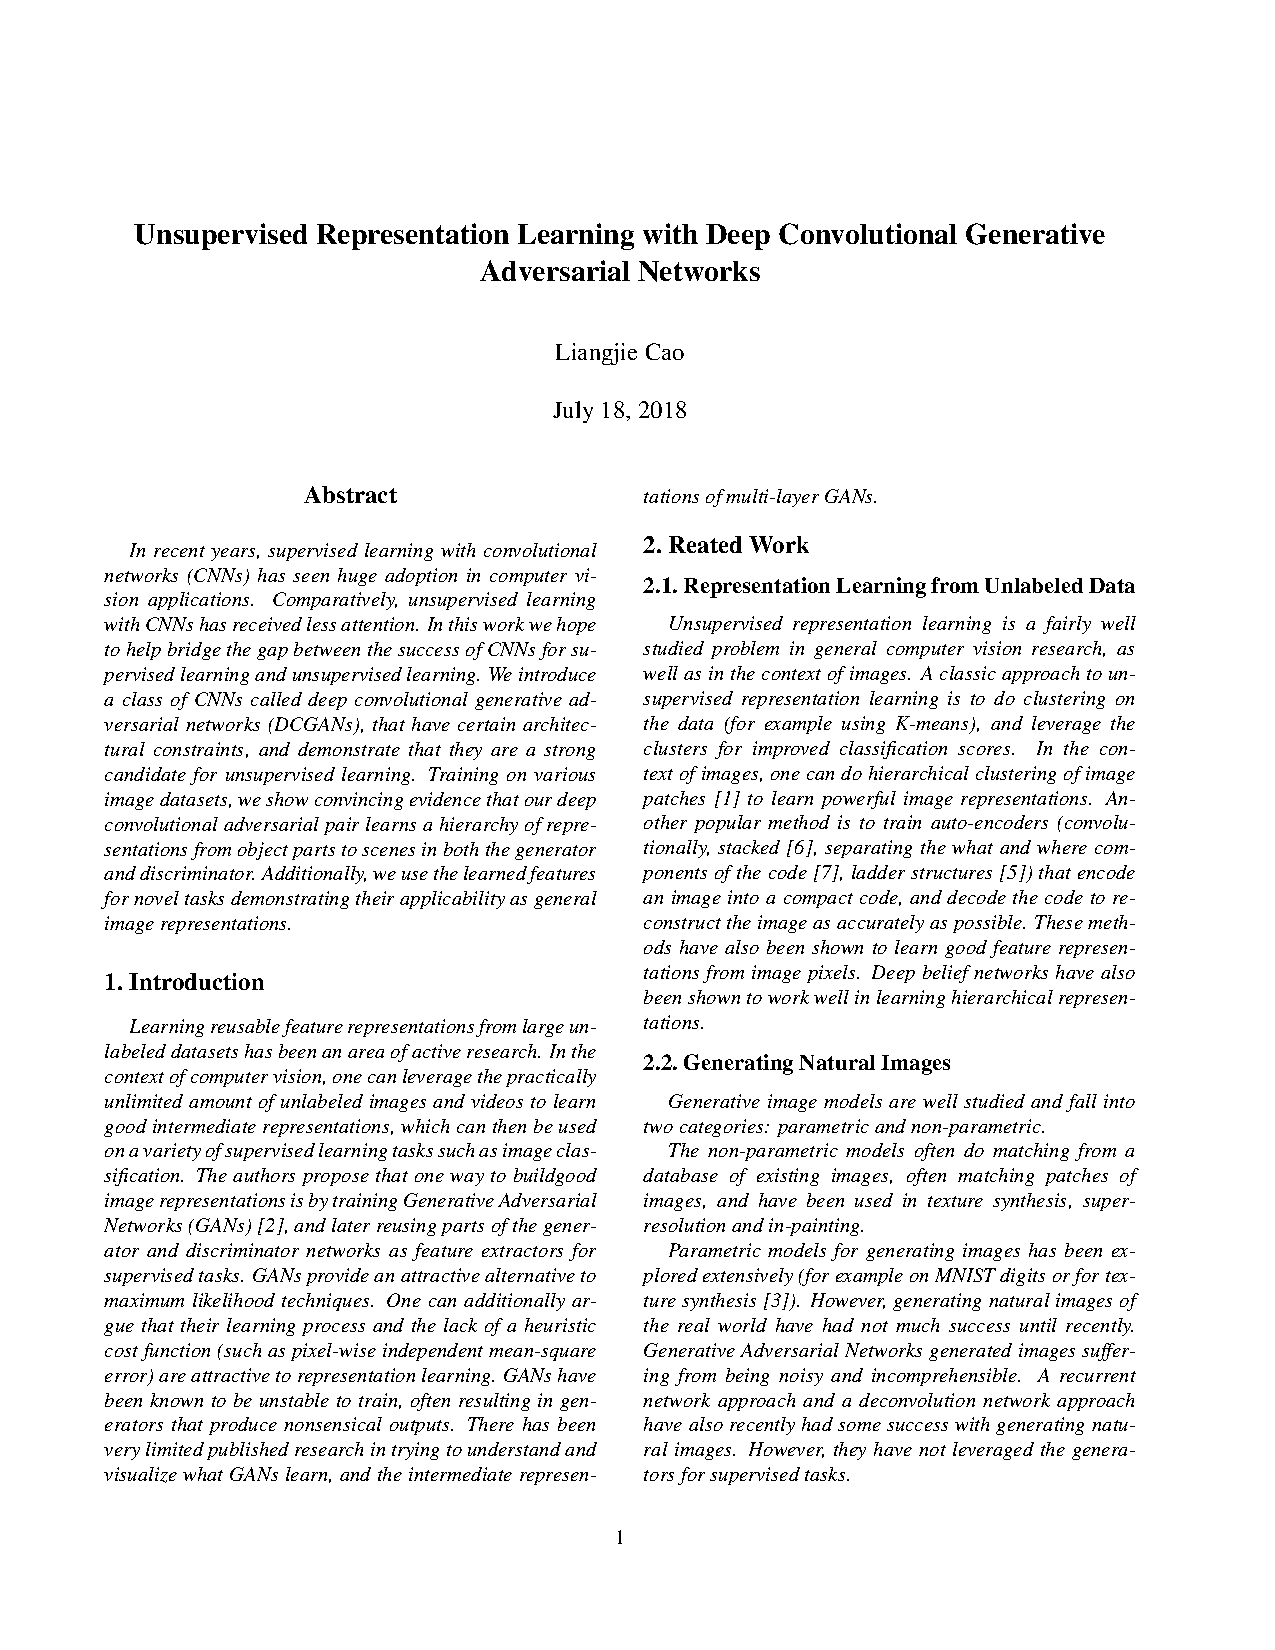
\includegraphics[width=3in]{DCGAN.png}\\
   	\caption{DCGAN generator used for LSUN scene modeling. A 100 dimensional uniform distribution Z is projected to a small spatial extent convolutional representation with many feature maps. A series of four fractionally-strided convolutions (in some recent papers, these are wrongly called deconvolutions) then convert this high level representation into a 64 x 64 pixel image. Notably, no fully connected or pooling layers are used}\label{Figure1}
   \end{figure}
\par A middle ground of directly connecting the highest
convolutional features to the input and output respectively of the generator and discriminator worked well. The first layer of the GAN, which takes a uniform noise distribution $Z$ as input, could be called
fully connected as it is just a matrix multiplication, but the result is reshaped into a 4D tensor and used as the start of the convolution stack. For the discriminator, the last convolution layer is flattened and then fed into a single sigmoid output. See Fig~\ref{Figure1} for a visualization of an example model architecture.   
\bibliographystyle{abbrv}
\bibliography{yinyong11}
\end{document}